% (find-LATEX "2020-1-C3-superficies-1.tex")
% (defun c () (interactive) (find-LATEXsh "lualatex -record 2020-1-C3-superficies-1.tex" :end))
% (defun D () (interactive) (find-pdf-page      "~/LATEX/2020-1-C3-superficies-1.pdf"))
% (defun d () (interactive) (find-pdftools-page "~/LATEX/2020-1-C3-superficies-1.pdf"))
% (defun e () (interactive) (find-LATEX "2020-1-C3-superficies-1.tex"))
% (defun u () (interactive) (find-latex-upload-links "2020-1-C3-superficies-1"))
% (defun v () (interactive) (find-2a '(e) '(d)) (g))
% (find-pdf-page   "~/LATEX/2020-1-C3-superficies-1.pdf")
% (find-sh0 "cp -v  ~/LATEX/2020-1-C3-superficies-1.pdf /tmp/")
% (find-sh0 "cp -v  ~/LATEX/2020-1-C3-superficies-1.pdf /tmp/pen/")
%   file:///home/edrx/LATEX/2020-1-C3-superficies-1.pdf
%               file:///tmp/2020-1-C3-superficies-1.pdf
%           file:///tmp/pen/2020-1-C3-superficies-1.pdf
% http://angg.twu.net/LATEX/2020-1-C3-superficies-1.pdf
% (find-LATEX "2019.mk")

% «.defs»		(to "defs")
% «.title»		(to "title")
% «.sombrero»		(to "sombrero")
% «.postes»		(to "postes")
% «.exercicio-1»	(to "exercicio-1")
% «.dica-cabos»		(to "dica-cabos")
% «.exercicio-2»	(to "exercicio-2")

\documentclass[oneside,12pt]{article}
\usepackage[colorlinks,citecolor=DarkRed,urlcolor=DarkRed]{hyperref} % (find-es "tex" "hyperref")
\usepackage{amsmath}
\usepackage{amsfonts}
\usepackage{amssymb}
\usepackage{pict2e}
\usepackage[x11names,svgnames]{xcolor} % (find-es "tex" "xcolor")
\usepackage{colorweb}                 % (find-es "tex" "colorweb")
%\usepackage{tikz}
%
% (find-dn6 "preamble6.lua" "preamble0")
%\usepackage{proof}   % For derivation trees ("%:" lines)
%\input diagxy        % For 2D diagrams ("%D" lines)
%\xyoption{curve}     % For the ".curve=" feature in 2D diagrams
%
\usepackage{edrx15}               % (find-LATEX "edrx15.sty")
\input edrxaccents.tex            % (find-LATEX "edrxaccents.tex")
\input edrxchars.tex              % (find-LATEX "edrxchars.tex")
\input edrxheadfoot.tex           % (find-LATEX "edrxheadfoot.tex")
\input edrxgac2.tex               % (find-LATEX "edrxgac2.tex")
%
%\usepackage[backend=biber,
%   style=alphabetic]{biblatex}            % (find-es "tex" "biber")
%\addbibresource{catsem-slides.bib}        % (find-LATEX "catsem-slides.bib")
%
% (find-es "tex" "geometry")
\usepackage[a6paper, landscape,
            top=1.5cm, bottom=.25cm, left=1cm, right=1cm, includefoot
           ]{geometry}
%
\begin{document}

\catcode`\^^J=10
\directlua{dofile "dednat6load.lua"}  % (find-LATEX "dednat6load.lua")

%L dofile "edrxtikz.lua"  -- (find-LATEX "edrxtikz.lua")
%L dofile "edrxpict.lua"  -- (find-LATEX "edrxpict.lua")
\pu

% «defs»  (to ".defs")
% (find-LATEX "edrx15.sty" "colors-2019")
\long\def\ColorRed   #1{{\color{Red1}#1}}
\long\def\ColorViolet#1{{\color{MagentaVioletLight}#1}}
\long\def\ColorViolet#1{{\color{Violet!50!black}#1}}
\long\def\ColorGreen #1{{\color{SpringDarkHard}#1}}
\long\def\ColorGreen #1{{\color{SpringGreenDark}#1}}
\long\def\ColorGreen #1{{\color{SpringGreen4}#1}}
\long\def\ColorGray  #1{{\color{GrayLight}#1}}
\long\def\ColorGray  #1{{\color{black!30!white}#1}}
\long\def\ColorBrown #1{{\color{Brown}#1}}
\long\def\ColorBrown #1{{\color{brown}#1}}

\long\def\ColorShort #1{{\color{SpringGreen4}#1}}
\long\def\ColorLong  #1{{\color{Red1}#1}}

\def\frown{\ensuremath{{=}{(}}}
\def\True {\mathbf{V}}
\def\False{\mathbf{F}}

\def\drafturl{http://angg.twu.net/LATEX/2020-1-C2.pdf}
\def\drafturl{http://angg.twu.net/2020.1-C2.html}
\def\draftfooter{\tiny \href{\drafturl}{\jobname{}} \ColorBrown{\shorttoday{} \hours}}


%  _____ _ _   _                               
% |_   _(_) |_| | ___   _ __   __ _  __ _  ___ 
%   | | | | __| |/ _ \ | '_ \ / _` |/ _` |/ _ \
%   | | | | |_| |  __/ | |_) | (_| | (_| |  __/
%   |_| |_|\__|_|\___| | .__/ \__,_|\__, |\___|
%                      |_|          |___/      
%
% «title»  (to ".title")
% (c3m201sups1p 1 "title")
% (c3m201sups1a   "title")

\thispagestyle{empty}

\begin{center}

\vspace*{1.2cm}

{\bf \Large Cálculo 3 - 2020.1}

\bsk

Aulas 9 e 10: introdução a superfícies e curvas de nível

\bsk

Eduardo Ochs - RCN/PURO/UFF

\url{http://angg.twu.net/2020.1-C3.html}

\end{center}

\newpage

\vspace*{2cm}

{\footnotesize

Obs: nós começamos a aula de hoje fazendo os exercícios 4 e 5

da aula passada, que ninguém tinha conseguido terminar... Link:

\ssk

\url{http://angg.twu.net/LATEX/2020-1-C3-taylor-3.pdf}

}

\newpage

Nós estamos usando dois truques diferentes pra fazer esboços de
trajetórias. O primeiro truque foi calcular $P(t)$ para vários valores
de $t$ e aí ligar os pontos de algum jeito que nos pareça razoável; o
segundo foi usar $P(t_0), P'(t_0), P''(t_0), \ldots$ para conseguir
aproximações de primeira e de segunda ordem para a trajetória $P$ em
torno do instante $t_0$.

Nossos primeiros exercícios de hoje vão ser sobre como adaptar o
método do ``calcular $P(t)$ para vários valores de $t$ e aí ligar os
pontos de algum jeito que nos pareça razoável'' para funções
$F:\R^2→\R$.

Você vai precisar de papel -- eu vou supor que o seu papel está na
horizontal sobre uma mesa --, lápis, e um pouco de coordenação motora
e imaginação.

Desenhe os eixos $x$ e $y$ no papel de forma que cada unidade nos
eixos corresponda a 1cm -- por exemplo, o ponto $(1,0)$ deve estar a
1cm do ponto $(0,0)$. Desenhe um quadriculado se isso te ajudar.

\newpage

% «sombrero»  (to ".sombrero")
% (c3m201sups1p 5 "sombrero")
% (c3m201sups1a   "sombrero")

Pegue algum objeto bem pontudo, como por exemplo uma caneta ou uma
faca de ponta. Você vai usar ele pra apontar pontos em $\R^3$.
\ColorRed{O eixo $z$ vai apontar fora do papel e pra cima.} Os pontos
de $\R^3$ com $z=0$, como $(3,2,0)$, vão estar exatamente sobre o
papel. Os pontos de $\R^3$ com $z=1$, como $(3,2,1)$, vão estar
flutuando exatamente 1cm acima sobre o papel -- e o ponto $(3,2,1)$
vai estar exatamente 1cm acima do ponto $(3,2,0)$.

É beeeem difícil desenhar à mão superfícies como o ``sombrero'' que eu
usei como exemplo no início da aula 5 -- link:

\ssk

\url{http://angg.twu.net/LATEX/2020-1-C3-taylor-2.pdf}

\ssk


\noindent
...mas é bem fácil desenhar versões super-low-tech dessas superfícies
de um jeito que \ColorRed{eu, você e os seus colegas que estão fazendo
  este curso de Cálculo 3 com você} entendam.


\newpage

% (c3m201taylor2p 2 "sombrero")
% (c3m201taylor2    "sombrero")

O sombrero da aula 5 era esta superfície:
%
$$S = \setofst{(x,y,x)}{r = \sqrt{x^2 + y^2}, z = \sen(r)/r}:$$
%
% (find-node "(octave)Three-Dimensional Plots" "sombrero")
% (find-fline "/usr/share/info/mesh.png")
% (find-fline "~/LATEX/2020-1-C3/")
% (find-latexgimp-links "2020-1-C3/mesh")
% (find-fline   "~/LATEX/2020-1-C3/mesh.png")
$$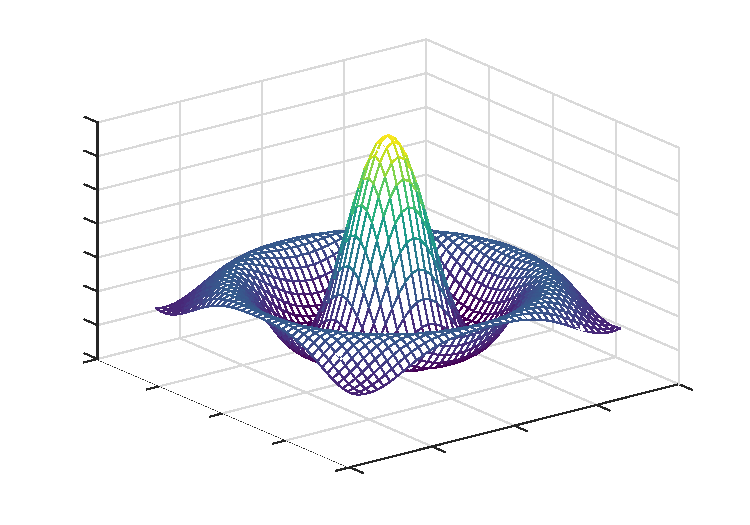
\includegraphics[height=4cm]{2020-1-C3/mesh.png}$$


\newpage

% «postes»  (to ".postes")
% (c3m201sups1p 6 "postes")
% (c3m201sups1    "postes")

{\bf Postes}

\ssk

Vamos começar com um exemplo mais simples que o sombrero, e que quase
todo mundo deve ter visto no final do curso de Geometria Analitica.
Seja $F(x,y) = x^2+y^2$ e vamos tentar visualizar o parabolóide
%
$$P = \setofst{(x,y,z)∈\R^2}{z=F(x,y)}.$$

Por exemplo, para $(x,y) = (3,2)$ temos $F(x,y) = 3^2+2^2 = 13$, e o
ponto da superfície $P$ que tem $x=3$ e $y=2$ é o ponto no qual
$z=13$... isto é, é o ponto $(3,2,13)$, que está 13cm acima do ponto
$(3,2,0)$, que está na superfície do papel.

Vamos representar isso graficamente escrevendo o número ``13'' no
ponto $(3,2)$ do nosso plano $(x,y)$. Esse número 13 vai querer dizer
``\ColorRed{imagine que tem um poste de 13cm aqui feito de madeira
  infinitamente fina. O ponto no topo deste poste pertence à nossa
  superfície}''.


\newpage

{\bf Postes (2)}

\ssk

Se escrevermos a altura dos postes em vários pontos de $\R^2$ com
coordenadas inteiras vamos obter o desenho abaixo à esquerda... e se a
nossa função fosse $F(x,y)=xy$ obteríamos o desenho abaixo à direita
-- \ColorRed{em que alguns postes têm altura negativa}.


% (find-LATEX "material-para-GA.tex" "pictureFxy")

\unitlength=15pt

\def\tcell#1{\lower\celllower\hbox to 0pt{\hss\cellfont#1\hss}}
\def\pictureFxy(#1,#2)(#3,#4)#5{%
  \vcenter{\hbox{%
  \beginpictureb(#1,#2)(#3,#4){.7}%
  {\color{GrayPale}%
   \Line(#1,0)(#3,0)%
   \Line(0,#2)(0,#4)%
  }
  \expr{pictFxy("#5")}
  \end{picture}%
  }}%
}


% (mpgp 24 "Fxy")
% (mpg     "Fxy")


\def\smF#1{\sm{F(x,y) \\ #1} ⇒}

$\smF{\;\;\;=\,x^2+y^2}
 \pictureFxy(-3,-2)(3,2){x*x+y*y}
 \quad
 \smF{\;\;\;=\,xy}
 \pictureFxy(-3,-3)(3,3){x*y}
$

\newpage

{\bf Postes (2)}

\ssk

O sombrero do slide 5 foi desenhado exatamente por este método. Pra um
certo grid de pontos $(x,y)∈\R^2$ um programa calculou a altura do
poste em cada ponto -- e depois desenhos cabos grossos ligando o ponto
no topo de cada poste aos pontos no topo dos postes acima, abaixo, à
direita e à esquerda dele.


\newpage

% «exercicio-1»  (to ".exercicio-1")
% (c3m201sups1p 9 "exercicio-1")
% (c3m201sups1    "exercicio-1")

{\bf Exercício 1.}

\ssk

a) Faça o ``diagrama de numerozinhos'' (como os que acabamos de fazer)
para a função $F(x,y) = (x+y)·y$.

\msk

b) Leia o início da seção 3.3 do Bortolossi (no capítulo 3) e entenda o
conceito de curvas de nível. Faça o exercício 24 da página 113 do
capítulo 3. Repare que ele dá a fórmula para cada superfício só por
curiosidade -- o importante neste exercício é só a gente aprender a
relacionar superfícies desenhadas do jeito 3D usual com as suas curvas
de nível.

\msk

c) (Continuação do item a) Faça as curvas de nível de $z=F(x,y) =
(x+y)·y$ para $z=0$, $z=1$ e $z=2$.


% (find-bortolossi3page (+ -78  97) "3.3. Curvas de nível")
% (find-bortolossi3page (+ -78  98)   "O desenho da curva de nível deve ser feito no plano")
% (find-bortolossi3page (+ -78 114)   "Curvas de nível de seis funções diferentes")
% (find-bortolossi3page (+ -78 115)   "Gráficos de seis funções diferentes")

\newpage

% «dica-cabos»  (to ".dica-cabos")
% (c3m201sups1p 10 "dica-cabos")
% (c3m201sups1     "dica-cabos")

{\bf Dica: use os cabos}

\ssk

Este é o diagrama de numerozinhos para $F(x,y)=x^2+y^2$:

\unitlength=12pt

\msk

$\smF{\;\;\;=\,x^2+y^2}
 \pictureFxy(-3,-2)(3,2){x*x+y*y}
$

Digamos que queremos usá-lo pra desenhar a curva de nível de $z=4$. Só
temos 4 postes com altura 4, e se só ligarmos estes 4 postes vamos ter
uma aproximação muito ruim pra curva de nível do $z=4$. Mas cada poste
com altura $2$ tem dois postes vizinhos a ele com altura 5, e você
pode marcar no olhômetro o ponto em que os cabos entre estes postes
passam pelo plano $z=4$. Fazendo isto você vai ter 12 pontos com
$z=4$, e ligando-os você consegue uma aproximação bem razoável para a
curva de nível que queremos.

\newpage

% «exercicio-2»  (to ".exercicio-2")
% (c3m201sups1p 11 "exercicio-2")
% (c3m201sups1     "exercicio-2")

{\bf Exercício 2.}

\ssk

Nas aulas passadas nós vimos como fazer algumas contas usando {\sl
  diferenciais}. Agora vamos fazer a mesma coisa com a função $F(x,y)
= (x+y)y$.

Digamos que $z=F(x,y)=(x+y)y$, $x=g(t)$, $y=h(t)$.

\msk

a) Calcule $\frac{dz}{dt}$. Você deve obter uma equação da forma
``$\frac{dz}{dt} = \ldots$'' onde a expressão ``$\ldots$'' só menciona
as variáveis $x$ e $y$ e as ``variáveis'' (entre aspas! Vamos entender
os detalhes disto depois) $\frac{dx}{dt}$ e $\frac{dy}{dt}$. Chame
esta equação de [a].

\ssk

b) Multiplique os dois lados da [a] por $dt$ para cancelar os
``$dt$''s. Obtenha uma igualdade da forma ``$dz = \ldots dx + \ldots
dy$'', onde cada ``$\ldots$'' só depende das variáveis $x$ e $y$.
Chame a equação ``$dz = \ldots dx + \ldots dy$'' que você obteve de
[b].

\newpage

{\bf Spoilers}

\ssk

Exercício 2b:

% (find-latexgimp-links "2020-1-C3/aula9_exercicio_2b")
% (find-fline   "~/LATEX/2020-1-C3/aula9_exercicio_2b.pdf")
$$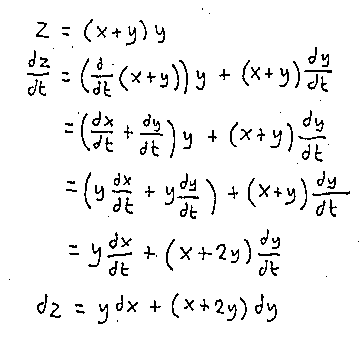
\includegraphics[height=6cm]{2020-1-C3/aula9_exercicio_2b.pdf}$$







%\printbibliography

\end{document}

%  __  __       _        
% |  \/  | __ _| | _____ 
% | |\/| |/ _` | |/ / _ \
% | |  | | (_| |   <  __/
% |_|  |_|\__,_|_|\_\___|
%                        
% <make>

 (eepitch-shell)
 (eepitch-kill)
 (eepitch-shell)
# (find-LATEXfile "2019planar-has-1.mk")
make -f 2019.mk STEM=2020-1-C3-superficies-1 veryclean
make -f 2019.mk STEM=2020-1-C3-superficies-1 pdf

% Local Variables:
% coding: utf-8-unix
% ee-tla: "c3m201sups1"
% End:
